\documentclass[mathserif,10pt]{beamer}
\usepackage[T1]{fontenc}
\usepackage{amsmath, amssymb}
\usepackage{times}
\usepackage{newtxtext}
\usepackage{algorithm}  
\usepackage{algorithmic} 
\usepackage{caption}
\usepackage{animate} 
\usepackage{lipsum} % just to generate dummy text

\usetheme[
%%% option passed to the outer theme
%    progressstyle=fixedCircCnt,   % fixedCircCnt, movingCircCnt (moving is deault)
  ]{Feather}
  
% If you want to change the colors of the various elements in the theme, edit and uncomment the following lines

% Change the bar colors:
%\setbeamercolor{Feather}{fg=red!20,bg=red}

% Change the color of the structural elements:
%\setbeamercolor{structure}{fg=red}

% Change the frame title text color:
%\setbeamercolor{frametitle}{fg=blue}

% Change the normal text color background:
%\setbeamercolor{normal text}{fg=black,bg=gray!10}

%-------------------------------------------------------
% INCLUDE PACKAGES
%-------------------------------------------------------

\usepackage[utf8]{inputenc}
\usepackage[english]{babel}
\usepackage[T1]{fontenc}
\usepackage{helvet}

%-------------------------------------------------------
% DEFFINING AND REDEFINING COMMANDS
%-------------------------------------------------------

% colored hyperlinks
\newcommand{\chref}[2]{
  \href{#1}{{\usebeamercolor[bg]{Feather}#2}}
}

%-------------------------------------------------------
% INFORMATION IN THE TITLE PAGE
%-------------------------------------------------------

\title[Mathematics in OI] % [] is optional - is placed on the bottom of the sidebar on every slide
{ % is placed on the title page
      \textbf{Mathematics in Olympiad in Informatics \\[0.3cm] Part 1}
}


\author[Haoyue Shi]
{      Frederica Haoyue Shi \\
      {\ttfamily hyshi@pku.edu.cn}
}

\institute[School of EECS, Peking University]
{
      School of Electronics Engineering and Computer Science\\
	  Peking University \\
  
  %there must be an empty line above this line - otherwise some unwanted space is added between the university and the country (I do not know why;( )
}

\date{\today}

%-------------------------------------------------------
% THE BODY OF THE PRESENTATION
%-------------------------------------------------------

\begin{document}

%-------------------------------------------------------
% THE TITLEPAGE
%-------------------------------------------------------

{\1% % this is the name of the PDF file for the background
\begin{frame}[plain,noframenumbering] % the plain option removes the header from the title page, noframenumbering removes the numbering of this frame only
  \titlepage % call the title page information from above
\end{frame}}


\begin{frame}{Content}{}
\tableofcontents
\end{frame}


%-------------------------------------------------------
\section{Introduction}
%-------------------------------------------------------
\begin{frame}{Introduction}
%-------------------------------------------------------
English is \textbf{very helpful} to our future study and work. Please try to use English as much as possible, from now on. 
\\~\\
Therefore, the slides are written in English. 
\\~\\
If there's no specific instruction, the complexity is always time complexity. 
\\~\\
For the convenience of view, I recommend you to open it with Adobe Reader. 
\end{frame}


%-------------------------------------------------------
\section{Number Theory}
\subsection{Division, Prime and Coprime}
%-------------------------------------------------------
\begin{frame}{Number Theory}{Division, Prime and Coprime}
%-------------------------------------------------------
\begin{block}{Fundamental theorem of arithmetic}
    Every integer greater than $1$ either is prime itself or is the product of prime numbers, and that this product is unique, up to the order of the factors. i.e. $$\forall n > 1, n \in \mathbb{N}, n = p_1^{a_1}p_2^{a_2} ... p_n^{a_n}$$ where $p_k (1\leq k\leq n), p_1<p_2<...<p_n$ is prime. 
\end{block}
\pause
\begin{block}{Prime Number Theorem}
    \begin{equation}
		\pi(N) \sim	 \frac{N}{\log(N)} \nonumber
	\end{equation}
	where $\pi(N)$ is the prime counting function, and $\log(N)$ is the natural logarithm of $N$. The equation means that for large enough $N$, the probability that a random natural number not greater than $N$ is prime is very close to $\frac{1}{\log(N)}$.
\end{block}
\end{frame}


%-------------------------------------------------------
\begin{frame}{Number Theory}{Division, Prime and Coprime}
%-------------------------------------------------------
\textbf{\large How to check whether a number $N$ is prime?}
\begin{algorithm}[H]
\begin{algorithmic}[1]
	\FOR{$i=2$ to $\sqrt{N}$}
		\IF{$i$ is divisor of $N$}
			\STATE \textbf{return} False
		\ENDIF
	\ENDFOR
\end{algorithmic}
\caption*{Pseudo-code for prime number checking.}
\end{algorithm}
\pause
~\\~\\
The time complexity of such algorithm is $O(\sqrt{N})$. \\
The space complexity of such algorithm is $O(1)$.

\end{frame}


%-------------------------------------------------------
\begin{frame}{Number Theory}{Division, Prime and Coprime}
%-------------------------------------------------------
\textbf{\large How to generate a prime number list from $1$ to $N$?}
\begin{enumerate}
	\item Check whether a number is prime one by one. \pause $O(N\sqrt{N})$ \pause
	\item Sieve of Eratosthenes 
\end{enumerate}
\end{frame}

%-------------------------------------------------------
\begin{frame}{Number Theory}{Division, Prime and Coprime}
%-------------------------------------------------------
\textbf{\large Sieve of Eratosthenes } \\
\begin{center}
\animategraphics[width=2in,height=2.2in,controls,loop]{10}{Images/output-}{0}{158}
\end{center}
\end{frame}


%-------------------------------------------------------
\begin{frame}{Number Theory}{Division, Prime and Coprime}
%-------------------------------------------------------
\textbf{\large How to generate a prime number list from $1$ to $N$?}
\begin{enumerate}
	\item Check whether a number is prime one by one. $O(N\sqrt{N})$
	\item Sieve of Eratosthenes \pause $O(N\log(N))$ \pause
	\item Linear Sieve
\end{enumerate}
\end{frame}


%-------------------------------------------------------
\begin{frame}{Number Theory}{Division, Prime and Coprime}
%-------------------------------------------------------
\begin{algorithm}[H]
\begin{algorithmic}[1]
	\FOR{$i=2$ to $N$}
		\STATE{set $IsPrime[i] = True$}
	\ENDFOR
	\FOR{$i=2$ to $N$}
		\IF{$IsPrime[i]$}
			\STATE{push $i$ into PrimeNumberList}
		\ENDIF
		\STATE{$j=0$}
		\WHILE{$j$ < CurrentPrimeNumber \textbf{and} $i \cdot $PrimeNumberList[$j$]$ < N$}
			\STATE{IsPrime[$i \cdot $PrimeNumberList[$j$]] = False}
			\IF{PrimeNumberList[$j$] is divisor of $i$}
				\STATE{\textbf{break}}
			\ENDIF
			\STATE{\textbf{increase} $j$}
		\ENDWHILE
	\ENDFOR
\end{algorithmic}
\caption*{Pseudo-code for linear sieve.}
\end{algorithm}
\end{frame}


%-------------------------------------------------------
\begin{frame}{Number Theory}{Division, Prime and Coprime}
%-------------------------------------------------------
\textbf{\large Linear Sieve} \\
The time complexity of such algorithm is $O(N)$. \\
The space complexity of such algorithm is $O(N)$. \\[0.5cm]
\pause
\textbf{Practice: POJ 2689} \\
Given $L, U(1\leq L < U < 2^{31}, U-L\leq 1,000,000)$, you are to find the two adjacent primes $C_1$ and $C_2 (L\leq C_1 < C_2 \leq U)$ that are closest (i.e. $C_2 - C_1$ is the minimum), and the two adjacent primes $D_1$ and $D_2 (L\leq D_1 < D_2 \leq U)$ that are the most distant (i.e. $D_2 - D_1$ is the maximum). 
\\~\\
\pause
Hint: You are definitely required to generate a prime number list in the range of $[L,U]$. But how?
\end{frame}


%-------------------------------------------------------
\begin{frame}{Optional: Mathematical Induction}
%-------------------------------------------------------
Mathematical induction is a mathematical proof technique used to prove a given statement about any well-ordered set. Most commonly, it is used to establish statements for the set of all natural numbers. \\~\\
\pause
It contains two steps:
\begin{enumerate}
\item \textbf{base case}, to prove the given statement for the least element in the well-ordered set. \pause
\item \textbf{inductive step}, to prove that, if the statement is assumed to be true for any element, then it must be true for the next element as well.
\end{enumerate}
\end{frame}

%-------------------------------------------------------
\begin{frame}{Optional: Mathematical Induction}
%-------------------------------------------------------
\textbf{\large An Example}
\\~\\
Prove $\sum_{i=0}^n = \frac{n(n+1)}{2}, \forall n\in \mathbb{N}$ \\[0.5cm]
\pause
\textbf{\sl Proof}~For the case $n=0$, we have $\sum_{i=0}^n=\frac{n(n+1)}{2}=0$. \\[0.2cm]
\pause
Assume that $\sum_{i=0}^n=\frac{n(n+1)}{2}$ when $n=k$, \\[0.2cm]
then $\sum_{i=0}^{k+1}=\frac{k(k+1)}{2}+k+1=\frac{k(k+1)+2(k+1)}{2}=\frac{(k+1)(k+2)}{2}$. \\[0.2cm]
Hence, the statement is true when $n=k+1$. \\[0.2cm]
\pause
Therefore, $\sum_{i=0}^n = \frac{n(n+1)}{2}, \forall n\in \mathbb{N}$. \#
\end{frame}


%-------------------------------------------------------
\begin{frame}{Number Theory}{Division, Prime and Coprime}
%-------------------------------------------------------
\textbf{\large Euclidean Algorithm for Greatest Common Divisor(GCD)}
\begin{algorithm}[H]
\begin{algorithmic}[1]
	\STATE{\textbf{function} GCD(\textbf{integer} a,b)}
	\IF{b == 0}
		\STATE{\textbf{return} a}
	\ELSE
		\STATE{\textbf{return} GCD(b, a \textbf{mod} b)}
	\ENDIF
\end{algorithmic}
\caption*{Pseudo-code for Euclidean Algorithm.}
\end{algorithm}

\pause
Most of you know how, but why?
\end{frame}

%-------------------------------------------------------
\begin{frame}{Number Theory}{Division, Prime and Coprime}
%-------------------------------------------------------
\textbf{\large Euclidean Algorithm for Greatest Common Divisor(GCD)}
\textbf{\sl Proof}  \\
For any two integers $a, b$, $a$ can be written as $$a = bq + r$$ where $q, r$ are non-negative integers, $0 \leq r < b$. \\ \pause
For all intergers $d$, if $d | a$ and $d | b$, then $$d|bq \Rightarrow d|(a-bq) \Rightarrow d|r$$ \pause
Namely, if $d$ is a common divisor of $a$ and $b$, then $d$ is a common divisor of $b$ and $r$, and vice versa. \\ \pause
Hence, GCD of $a$ and $b$ (denoted as $(a,b)$) equals $(b,r)$. \#
\end{frame}

%-------------------------------------------------------
\begin{frame}{Number Theory}{Division, Prime and Coprime}
%-------------------------------------------------------
\begin{block}{Bézout's Identity(Lemma)}
	Let $a$ and $b$ be nonzero integers and let $d$ be their greatest common divisor. Then there exist integers $x$ and $y$ such that $$ax+by=d$$ 
	In addition, 
	\begin{itemize}
		\item the greatest common divisor $d$ is the smallest positive integer that can be written as $ax + by$
		\item every integer of the form $ax + by$ is a multiple of the greatest common divisor $d$.
	\end{itemize}
\end{block}
~\\
It can be proved similarly to the proof of Euclidean Algorithm, and the so called Extended Euclidean Algorithm comes out.
\end{frame}

%-------------------------------------------------------
\begin{frame}{Number Theory}{Division, Prime and Coprime}
%-------------------------------------------------------
\textbf{\large Extended Euclidean Algorithm} \\[0.2cm]
Purpose: Given 3 intergers $a, b, c$, to find out all solutions for $$ax+by=c$$.
\begin{algorithm}[H]
\begin{algorithmic}[1]
	\STATE{\textbf{function} EX-EUC(\textbf{integer} a,b)}
	\IF{b == 0}
		\STATE{\textbf{set} x = 1, y = 0}
		\STATE{\textbf{return} a}
	\ELSE
		\STATE{\textbf{set} d = EX-EUC(b, a \textbf{mod} b)}
		\STATE{\textbf{set} t = x, x = y, y = t - a / b * y}
		\STATE{\textbf{return} d}
	\ENDIF
\end{algorithmic}
\caption*{Pseudo-code for Extended-Euclidean Algorithm}
\end{algorithm}
\end{frame}

%-------------------------------------------------------
\begin{frame}{Number Theory}{Division, Prime and Coprime}
%-------------------------------------------------------
\textbf{\large Extended Euclidean Algorithm} \\[0.2cm]
Purpose: Given 3 intergers $a, b, c$, to find out all solutions for $$ax+by=c$$.
\\[0.2cm]
Remember to check the case of NO SOLUTION : $d \nmid c$.
\end{frame}


%-------------------------------------------------------
\begin{frame}{Number Theory}{Division, Prime and Coprime}
%-------------------------------------------------------
\textbf{\large Practice: Compute $\sum_{i=1}^n K \bmod ~i,  1\leq K \leq 10^9$ } \\[0.5cm]
\pause
Hint:
$$K \bmod~i = K - \lfloor \frac{K}{i} \rfloor i$$
\pause 
For some successive $i$, $\lfloor \frac{K}{i} \rfloor$ remains constant. \\
\pause
How many such intervals are there, in the range of $[1, K]$? 
\pause ~~$O(\sqrt{K})$ 
~\\
Please finish the proof by yourselves and write the program after class. 
\end{frame}

%-------------------------------------------------------
\begin{frame}{Number Theory}{Division, Prime and Coprime}
%-------------------------------------------------------
\textbf{\large Euler's totient function}
$$
\phi(n) = n\prod_{p|n} (1-\frac{1}{p}) 
$$
where $p$ is a prime number.
\pause
~\\
Proof: Inclusion-Exclusion Principle
\pause
\begin{block}{Euler's Theorem}
If $n$ and $a$ are coprime positive integers, then
$$a^{\phi(n)} \equiv 1 (\bmod ~ n)$$
\end{block}
\end{frame}

%-------------------------------------------------------
\begin{frame}{Number Theory}{Division, Prime and Coprime}
%-------------------------------------------------------
\textbf{\large Proof of Euler's Theorem} \\
\textbf{\sl Proof} ~~ Let $R$ be a reduced residue system ($\bmod~ n$) and let $a$ be any integer coprime to $n$. \\
\pause
The proof hinges on the \textbf{fundamental fact} that multiplication by a permutes the sequence $\{x_i\}$: in other words if $ax_j \equiv ax_k (\bmod~n)$ then $j = k$. 
\\
\pause
That is, the sets $R$ and $aR = \{ax_1, ax_2, ..., ax_{\phi(n)}\}$. \\
\pause
Therefore, $$\prod_{i=1}^{\phi(n)}x_i \equiv \prod_{i=1}^{\phi(n)} ax_i \equiv a^{\phi(n)}\prod_{i=1}^{\phi(n)}x_i$$
\pause
$$\Rightarrow a^{\phi(n)} \equiv 1 (\bmod~n)$$
\end{frame}


%-------------------------------------------------------
\begin{frame}{Number Theory}{Congruence Modulo}
%-------------------------------------------------------
\begin{block}{Fermat's Little Theorem}
If $p$ is a prime number, then for any integer $a$, the number $a^p - a$ is an integer multiple of $p$. In the notation of modular arithmetic, this is expressed as
$$a^p \equiv a ~~(\bmod~ p)$$
\end{block}
\pause
Proof: Just a special case for Euler's Theorem. 
\end{frame}

\begin{frame}{Number Theory}{Congruence Modulo}
%-------------------------------------------------------
\textbf{\large Practice: POJ3090} \\
Write a program which, given a value for the size, $N$, computes the number of visible points $(x, y)$ with $0 \leq x, y \leq N$. $(1\leq N \leq 1000)$
\begin{center}
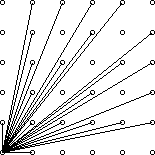
\includegraphics[width=0.2\linewidth]{Images/3090}
\end{center}
\pause
~\\ Hint: $GCD(x,y) = 1$
\end{frame}

%-------------------------------------------------------
\subsection{Congruence Modulo}
%-------------------------------------------------------
\begin{frame}{Number Theory}{Congruence Modulo}
%-------------------------------------------------------
\textbf{\large Modular multiplicative inverse} \\
This concept is analogous to the concept of the multiplicative inverse over the set of rational numbers.\\[0.5cm]
The modulo multiplicative inverse for the congruence class $\overline{a}$ is the congruence class $\overline{x}$ such that $\overline{a} \cdot \overline{x} \equiv 1 ~~(\bmod~~ m)$
\pause
~\\[0.2cm]
When a congruence class $\overline{a}$ has modulo multiplicative inverse?
\pause
~\\[0.2cm]
Answer: $(a, m) = 1$
\\[0.5cm]
\pause
Usage: Compute $\frac{a}{b} \bmod m$, where $(b, m) = 1$
\end{frame}


%-------------------------------------------------------
\begin{frame}{Number Theory}{Congruence Modulo}
%-------------------------------------------------------
\begin{block}{Chinese remainder theorem}
Assert $m_1, m_2, ..., m_k$ are pairwise coprime integers, $m = m_1m_2...m_k, M_i = \frac{m}{m_i}, M^{'}_iM_i\equiv 1(\bmod m_i), 1\leq i 
\leq k$, then there exists an integer $$x=\sum_{i=1}^k a_iM_i M^{'}_i$$ such that 

$$ x \equiv a_1 (\bmod~n_1) $$
$$ x \equiv a_2 (\bmod~n_2) $$
$$ ... $$
$$ x\equiv a_k (\bmod~n_k) $$
and any two $x$ are congruent modulo $M$.
\end{block}
\end{frame}


%-------------------------------------------------------
\section{Power and Matrix Multiplication}
\subsection{Exponentiation}
%-------------------------------------------------------
\begin{frame}{Power and Matrix Multiplication}{Exponentiation}
%-------------------------------------------------------
\textbf{\large Task: Compute $a ^ b$, a and b are non-negative integers.}
\begin{algorithm}[H]
\begin{algorithmic}[1]
\STATE{\textbf{set} result = 0}
\FOR{$i=1$ to $b$}
	\STATE{result = result $\cdot a$ }
\ENDFOR
\end{algorithmic}
\caption*{Pseudo-code for brute-force computing of $a^b$}
\end{algorithm}
\pause
The time complexity for the algorithm is $O(N)$. \\
The space complexity for the algorithm is $O(1)$.
\pause
Is there any faster algorithm? Yes.
\end{frame}


%-------------------------------------------------------
\begin{frame}{Power and Matrix Multiplication}{Exponentiation}
%-------------------------------------------------------
\textbf{\large Task: Compute $a ^ b$, a and b are non-negative integers.}
\begin{algorithm}[H]
\begin{algorithmic}[1]
\STATE{\textbf{function} power(a, b)}
\IF{b == 0}
	\STATE{\textbf{return} 1}
\ELSE
	\STATE{temp = power(a, b/2)}
	\STATE{result = temp$^2$}
	\IF{b $\bmod$  2 == 1}
		\STATE{result = result $\cdot$ a}
	\ENDIF
	\STATE{\textbf{return} result}
\ENDIF
\end{algorithmic}
\caption*{Pseudo-code for faster computing of $a^b$}
\end{algorithm}
\pause
Time Complexity: $O(\log N)$~~~~~~~Space Complexity: $O(\log N)$
\end{frame}

%-------------------------------------------------------
\subsection{Matrix Exponentiation}
\begin{frame}{Power and Matrix Multiplication}{Matrix Exponentiation}
%-------------------------------------------------------
\textbf{\large Matrix Multiplication}
$$A \times B = C $$
$$C_{ij} = \sum_k A_{ik} B_{kj}$$
\begin{center}
\pause
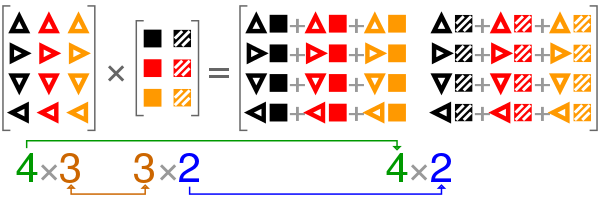
\includegraphics[width=0.8\linewidth]{Images/matrix}
\end{center}
\end{frame}

%-------------------------------------------------------
\begin{frame}{Power and Matrix Multiplication}{Matrix Exponentiation}
%-------------------------------------------------------
\textbf{\large Properties of Matrix Multiplication} \\[0.5cm]
\pause
Associative Law? \pause Yes. \\
\pause
Commutative Law? \pause \textbf{No!} \\[0.5cm]
We could apply fast exponentiation method to matrix multiplication to compute $A^n$ for a matrix $A$, but the code should be modify a little.
\end{frame}


%-------------------------------------------------------
\begin{frame}{Power and Matrix Multiplication}{Matrix Exponentiation}
%-------------------------------------------------------
\textbf{\large Task: Compute $A ^ b$, where $A$ is a matrix and b is a non-negative integer.}
\begin{algorithm}[H]
\begin{algorithmic}[1]
\STATE{\textbf{function} power(A, b)}
\IF{b == 0}
	\STATE{\textbf{return I}}
\ELSE
	\STATE{temp = power(A, b/2)}
	\STATE{result = temp$^2$}
	\IF{b $\bmod$  2 == 1}
		\STATE{result = result $\times$ A}
	\ENDIF
	\STATE{\textbf{return} result}
\ENDIF
\end{algorithmic}
\caption*{Pseudo-code for faster computing of $a^b$}
\end{algorithm}
\end{frame}

%-------------------------------------------------------
\begin{frame}{Power and Matrix Multiplication}{Matrix Exponentiation}
%-------------------------------------------------------
\textbf{\large Usage: Compute the $n^{th}$ item for Fibonacci Sequence.} \\[0.5cm]
Fibonacci Sequence: $f_0 = 1, f_1 = 1, f_n = f_{n-1} + f_{n-2} (k \geq 2)$ \\[0.5cm]
\begin{itemize}
	\item Enumerate every $i$ and compute $f_i$ one by one. \pause $O(n)$
	\pause
	\item Consider matrix multiplication:
	\begin{equation}
	\left(
	\begin{array}{cc}
		1 & 1 \\
		1 & 0
	\end{array}
	\right) \nonumber
	\end{equation}
	\\
	\pause $O(\log n) $
\end{itemize}
\end{frame}

%-------------------------------------------------------
\begin{frame}{Power and Matrix Multiplication}{Matrix Exponentiation}
%-------------------------------------------------------
\textbf{\large Why it works?} \\[0.5cm]
When we compute
\begin{equation}
	\left(
	\begin{array}{cc}
		1 & 1 \\
		1 & 0
	\end{array}
	\right) \times 
	\left(
	\begin{array}{c}
		1 \\
		1
	\end{array}
	\right) = 
	\left(
	\begin{array}{cc}
		2 \\
		1
	\end{array}
	\right)
	\nonumber
	\end{equation}
and
	\begin{equation}
	\left(
	\begin{array}{cc}
		1 & 1 \\
		1 & 0
	\end{array}
	\right) \times 
	\left(
	\begin{array}{c}
		2 \\
		1
	\end{array}
	\right) = 
	\left(
	\begin{array}{cc}
		3 \\
		2
	\end{array}
	\right)
	\nonumber
	\end{equation}
etc. \\
We actually did the recurrence procedure. Thus, according to the associative law of matrix multiplication, why not combine the exponentiation of the matrix in order to make the algorithm faster?
\end{frame}

%-------------------------------------------------------
\section{Linear Algebra}
\section{Probability and Expectation}
\section{Combinatorics}
\section{Introduction to Calculus}
\subsection{Differential of a Function}
\subsection{Calculus}
%-------------------------------------------------------




{\1
\begin{frame}[plain,noframenumbering]
  \finalpage{Part 1 ends here. Thank you for attention! \\ Powereed by \LaTeX. }
\end{frame}}

\end{document}